\documentclass{article}
    \usepackage[margin=0.8in]{geometry}
    \usepackage[parfill]{parskip}
    \usepackage[utf8]{inputenc}
    \usepackage{graphicx}
    \usepackage{siunitx}


\begin{document}
Excercise 5 \\
Rendell Cale, \today 


\section{}
The echo request was sent from src 192.168.1.102 to dst 128.59.23.100, so the clients IP address was 192.168.1.102. 
\begin{centering}
	\center
	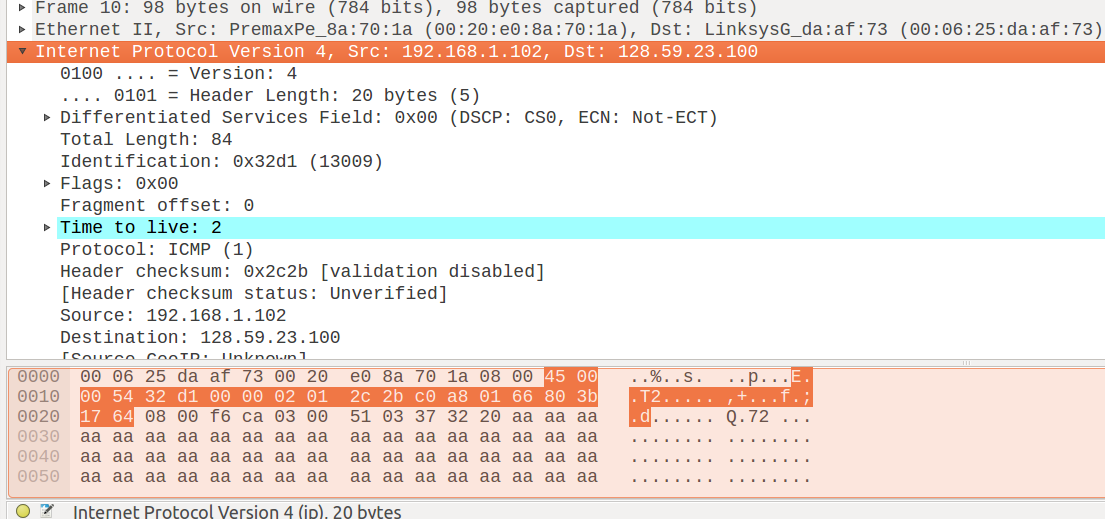
\includegraphics[width=\linewidth]{ip-header.png}
\end{centering}

\section{}
Clicking on the the message and pressing the Internet Protocol Version 4 tab highlights the header bytes. Counting them up show that the IPv4 header has \underline{20 bytes}, which corresponds well with what we would expect. This is also illustrated by the screenshot above. 

\section{}
The IP datagram has a payload of size \underline{64 bytes} which is the ICMP.

\begin{centering}
	\center
	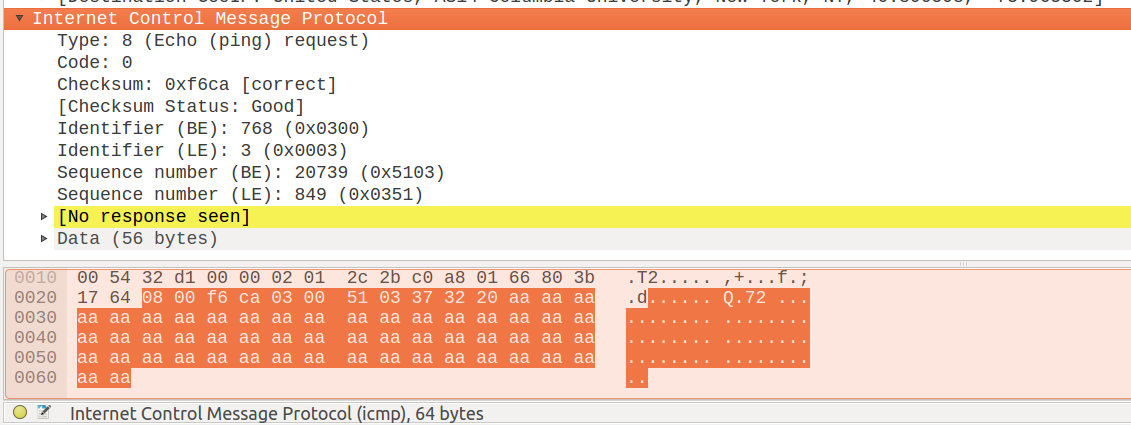
\includegraphics[width=\linewidth]{ip-datagram.png}
\end{centering}

\section{}
The IP header has none of the flags set and a fragmentation offset equal to zero. Thus the packet was \underline{not fragmenteed}. This makes sense since the payload is quite small, and it is using ethernet. 

\section{}
In the IP header we see that the fields "Identification", "Time to live", and of course "Header checksum" always change. 
In the ICMP part we see that the two sequence numbers (BE and LE) change, and also the chacksum. 

\section{}
In the header, the most interesting contant fields are source, destination, but note also that the vesion field, header length, differentiated services field, flags, and protocol fields are also constant.
The total length and fragment offset does change but infrequently. 

In the ICMP, the type is consistently 8 (Echo (ping) request) and code is 0. The identifiers also never change for both BE and LE. 

\section{}
The value in the identification field is ??

\section{}
TTL value is 255.


\end{document}
